%%
%% Class homework & solution template for latex
%% Alex Ihler
%%
\documentclass[twoside,11pt]{article}
\usepackage{amsmath,amsfonts,amssymb,amsthm}
\usepackage{graphicx,color}
\usepackage{verbatim,url}
\usepackage{listings}
\usepackage{upquote}
\usepackage[T1]{fontenc}
%\usepackage{lmodern}
\usepackage[scaled]{beramono}
\usepackage{enumerate}
\usepackage{float}
%\usepackage{textcomp}

% Directories for other source files and images
\newcommand{\bibtexdir}{../bib}
\newcommand{\figdir}{figs}

\newcommand{\E}{\mathrm{E}}
\newcommand{\Var}{\mathrm{Var}}
\newcommand{\N}{\mathcal{N}}
\newcommand{\matlab}{{\sc Matlab}\ }

\setlength{\textheight}{9in} \setlength{\textwidth}{6.5in}
\setlength{\oddsidemargin}{-.25in}  % Centers text.
\setlength{\evensidemargin}{-.25in} %
\setlength{\topmargin}{0in} %
\setlength{\headheight}{0in} %
\setlength{\headsep}{0in} %

\renewcommand{\labelenumi}{(\alph{enumi})}
\renewcommand{\labelenumii}{(\arabic{enumii})}

\theoremstyle{definition}
\newtheorem{MatEx}{M{\scriptsize{ATLAB}} Usage Example}

\definecolor{comments}{rgb}{0,.5,0}
\definecolor{backgnd}{rgb}{.95,.95,.95}
\definecolor{string}{rgb}{.2,.2,.2}
\lstset{language=Matlab}
\lstset{basicstyle=\small\ttfamily,
        mathescape=true,
        emptylines=1, showlines=true,
        backgroundcolor=\color{backgnd},
        commentstyle=\color{comments}\ttfamily, %\rmfamily,
        stringstyle=\color{string}\ttfamily,
        keywordstyle=\ttfamily, %\normalfont,
        showstringspaces=false}
\newcommand{\matp}{\mathbf{\gg}}




\begin{document}

\centerline{\Large Kyle Benson}
\centerline{CS 273A - Machine Learning: Fall 2013}
\centerline{Homework 5}

% % % % % % % % % % % % % % % % % % % % % % % % % % % % % % % % % % % % % % % % % % % % % % % % % % % % %
\subsection*{Problem 1: Basics of Clustering}

\begin{enumerate}[(a)]

\item TODO
%\item Polynomial training errors:
%\begin{figure}[h!] \centering
%\begin{tabular}{cccc}
%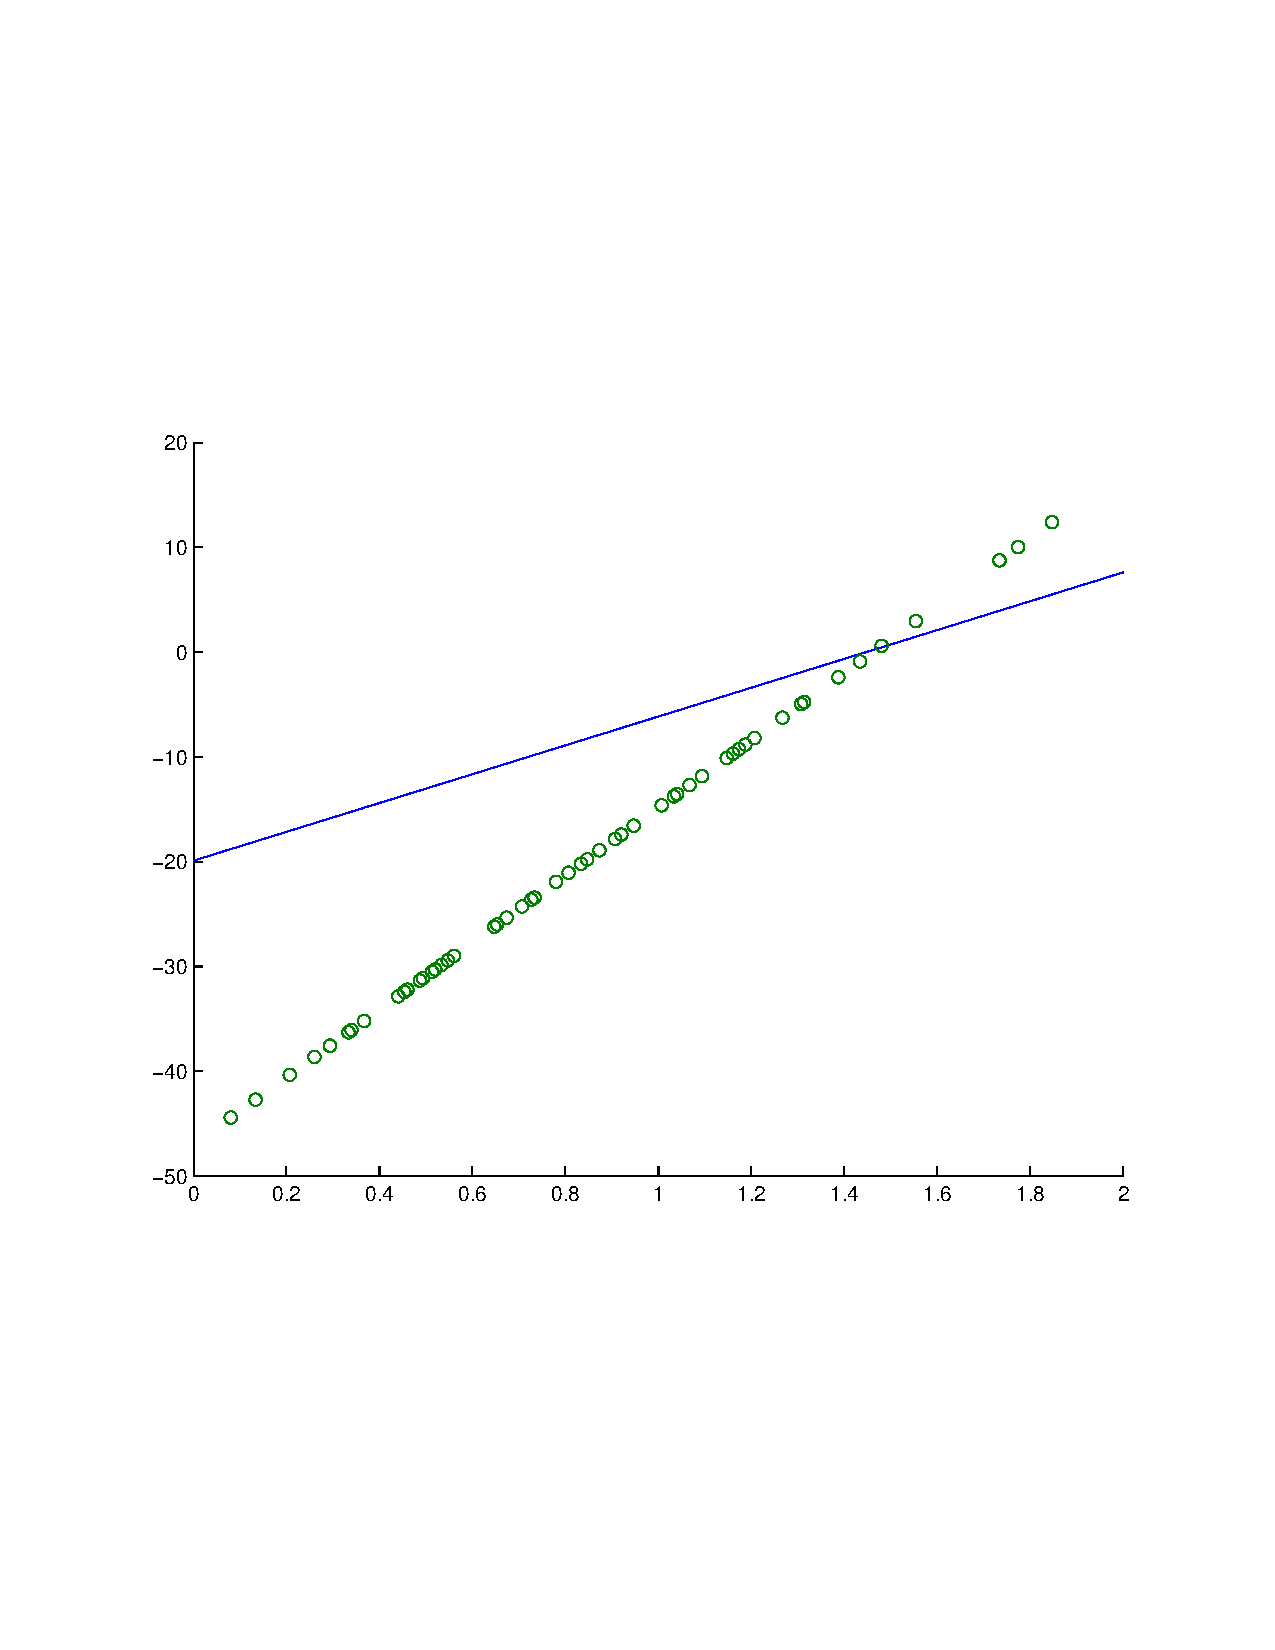
\includegraphics[width=.22\textwidth]{\figdir/prob1c_deg1} &
%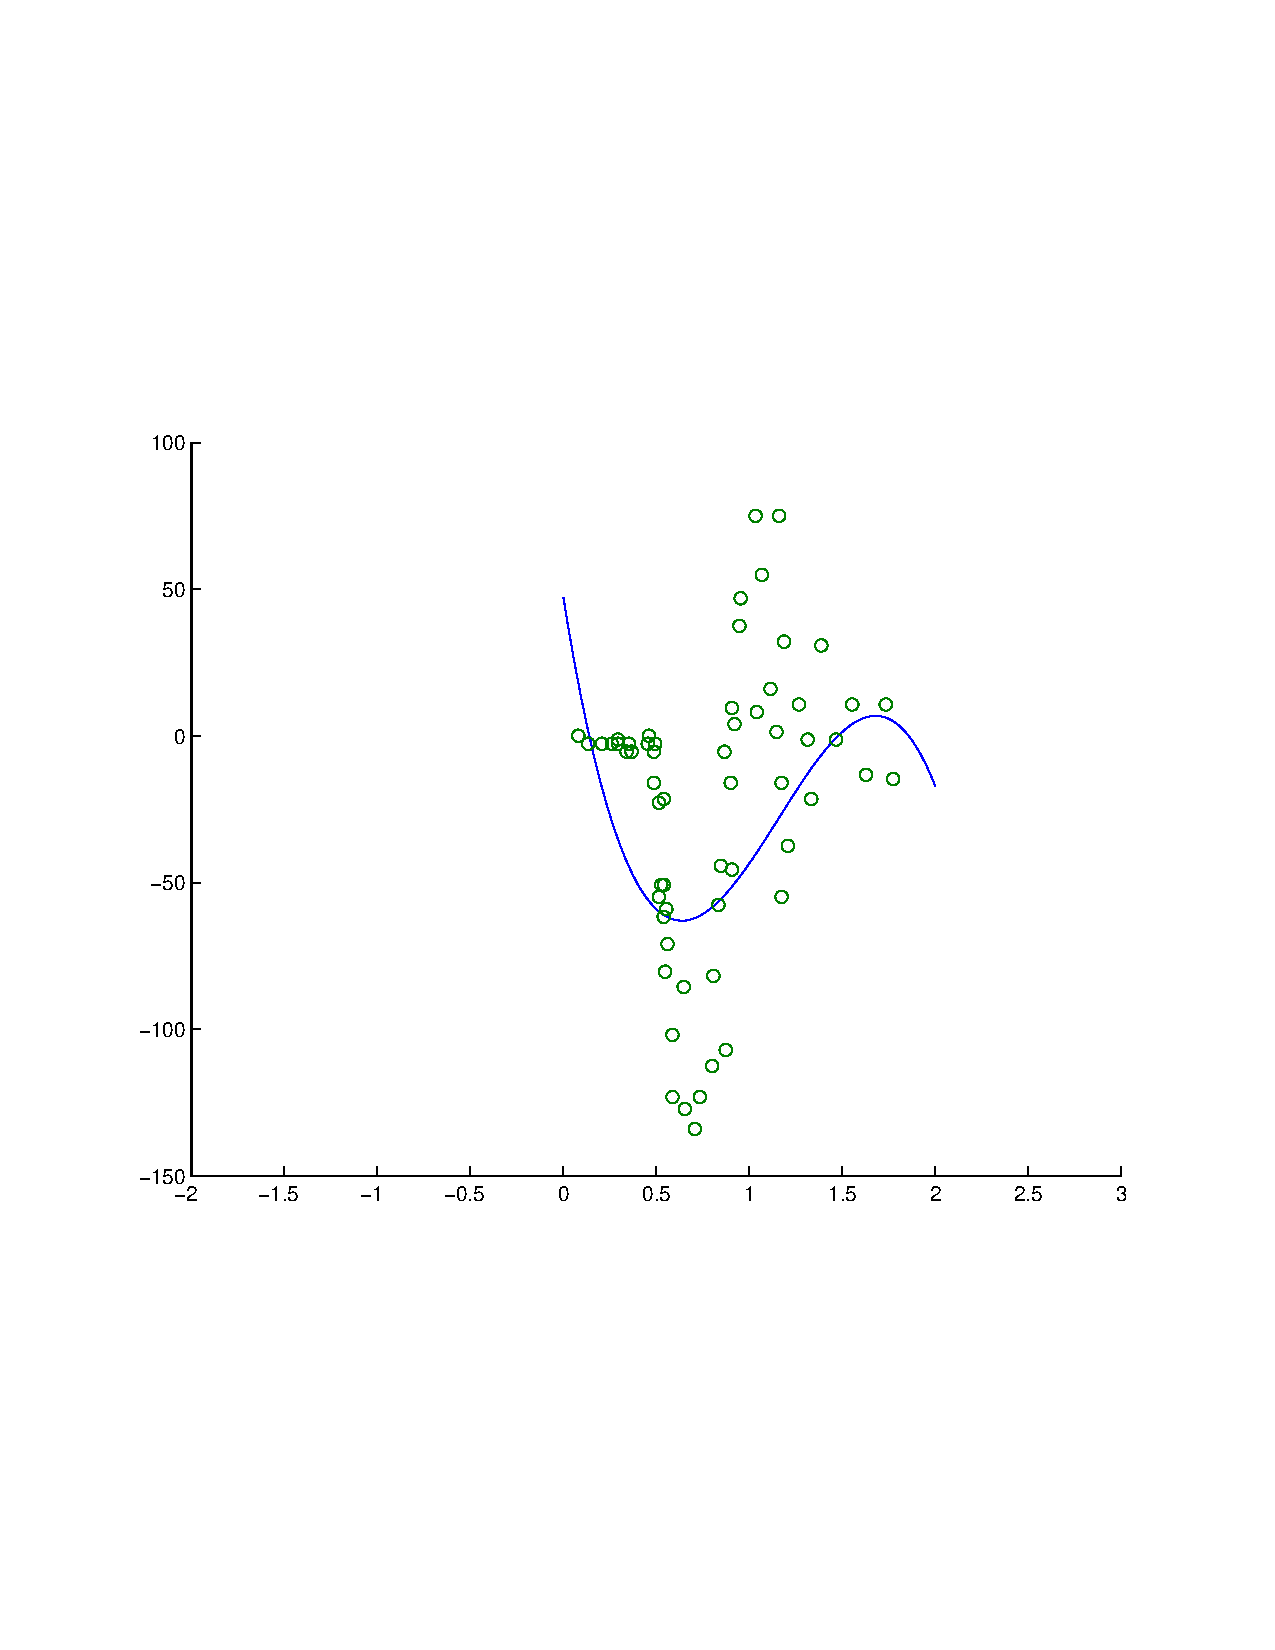
\includegraphics[width=.22\textwidth]{\figdir/prob1c_deg3} &
%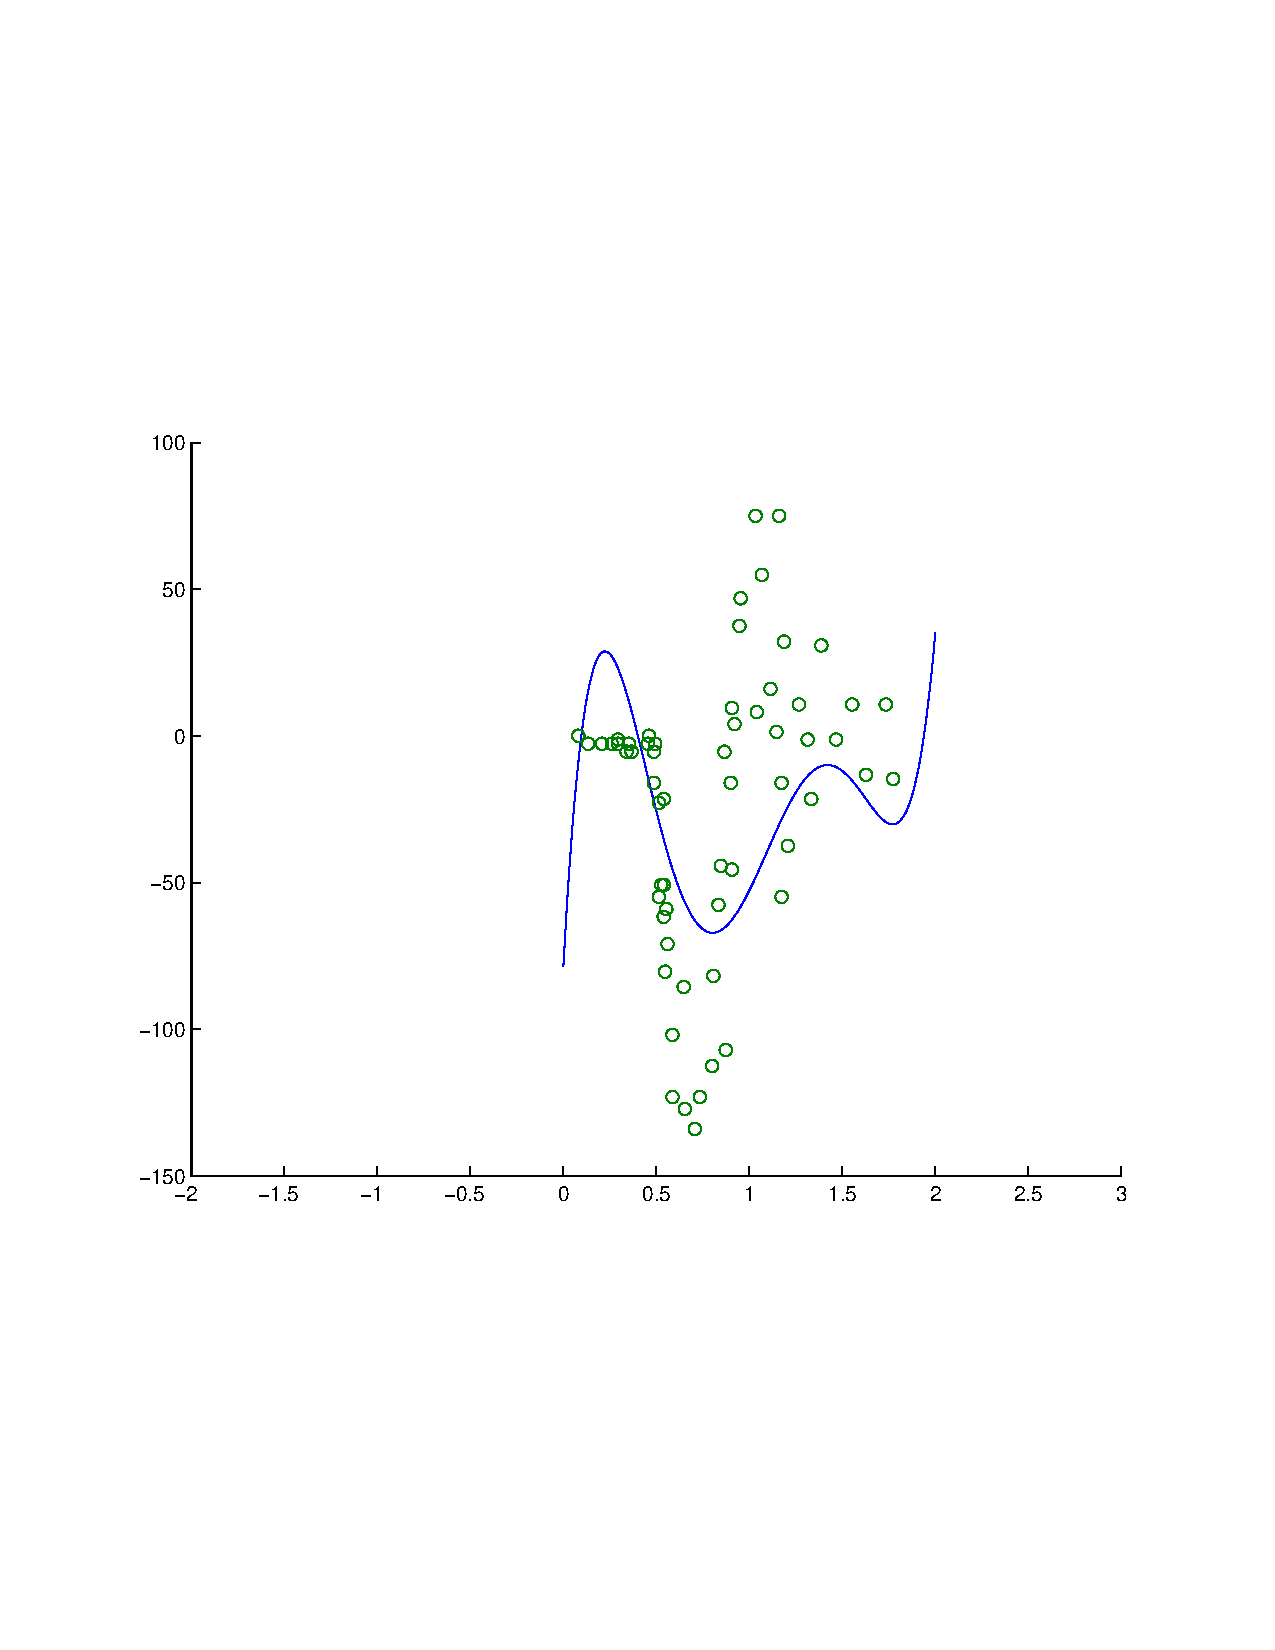
\includegraphics[width=.22\textwidth]{\figdir/prob1c_deg5} &
%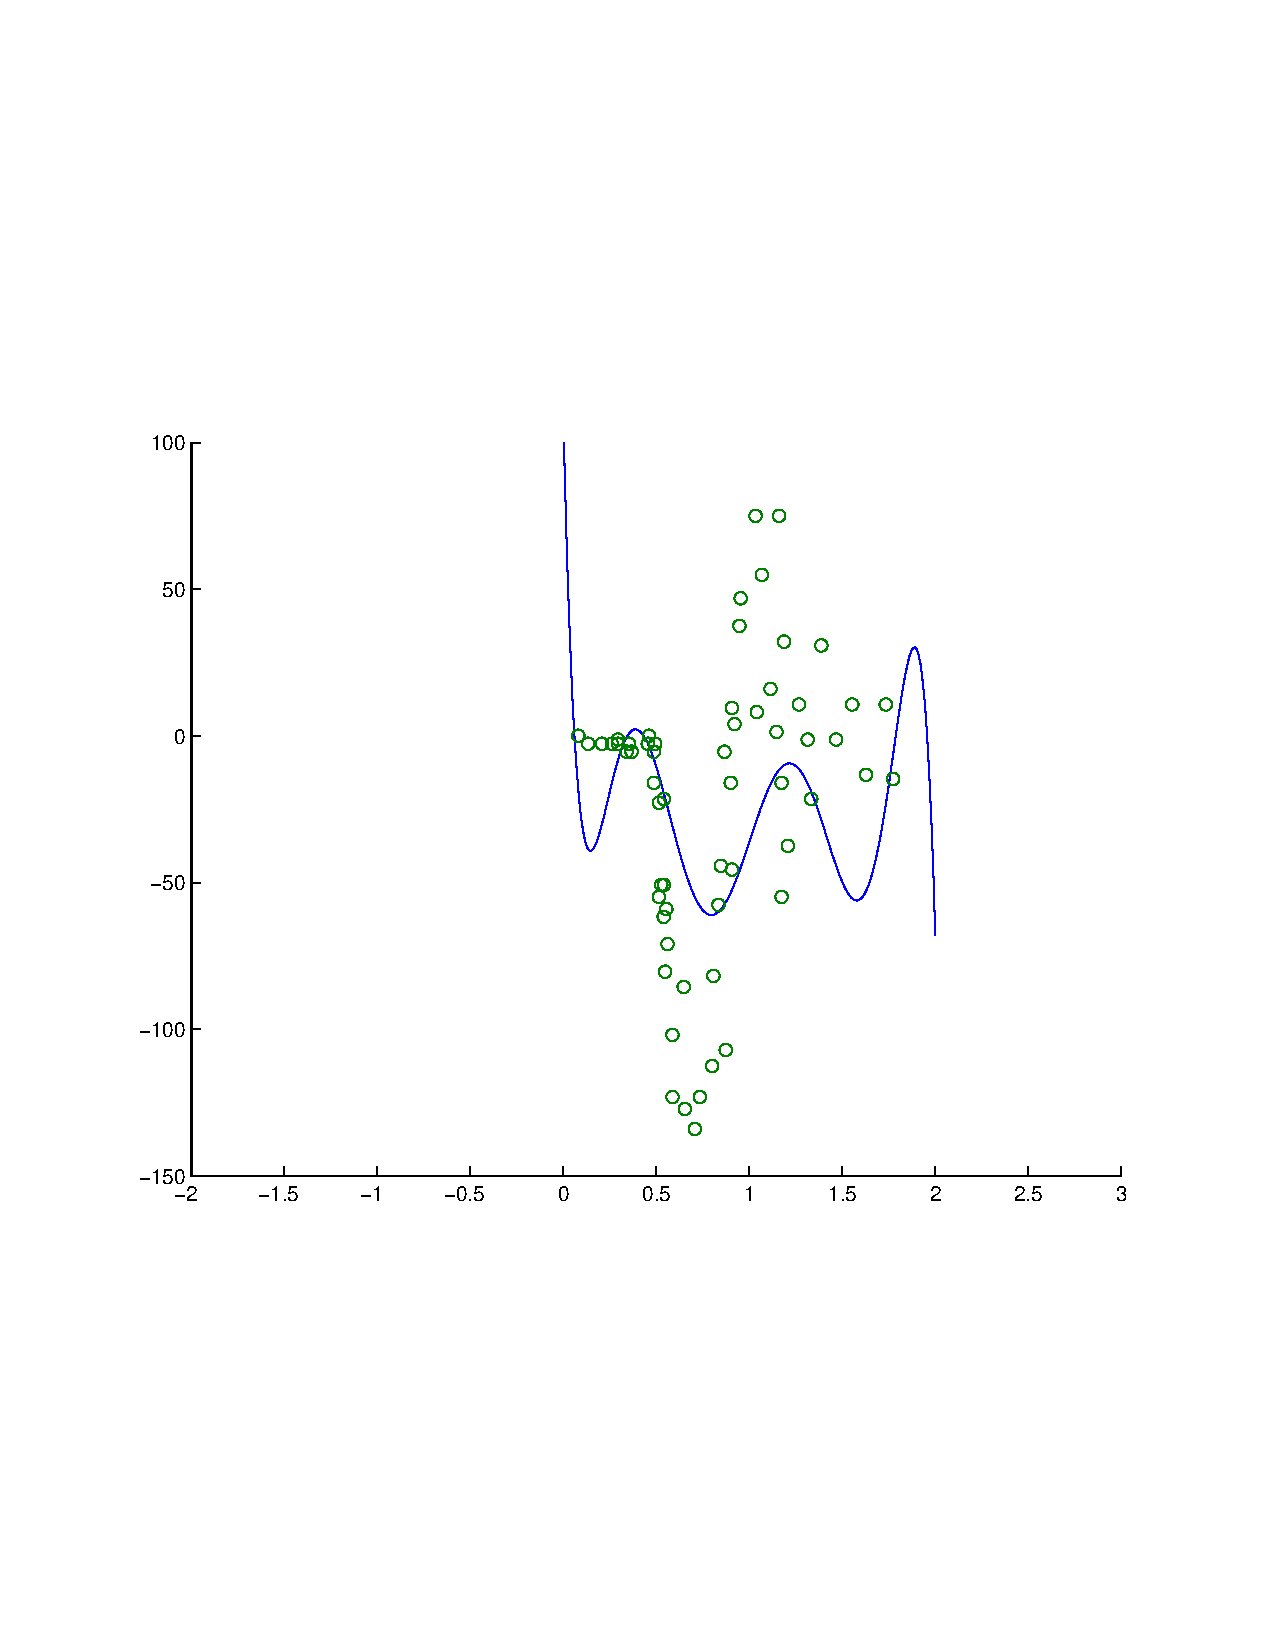
\includegraphics[width=.22\textwidth]{\figdir/prob1c_deg7} \\
%1 & 3 & 5 & 7 \\
%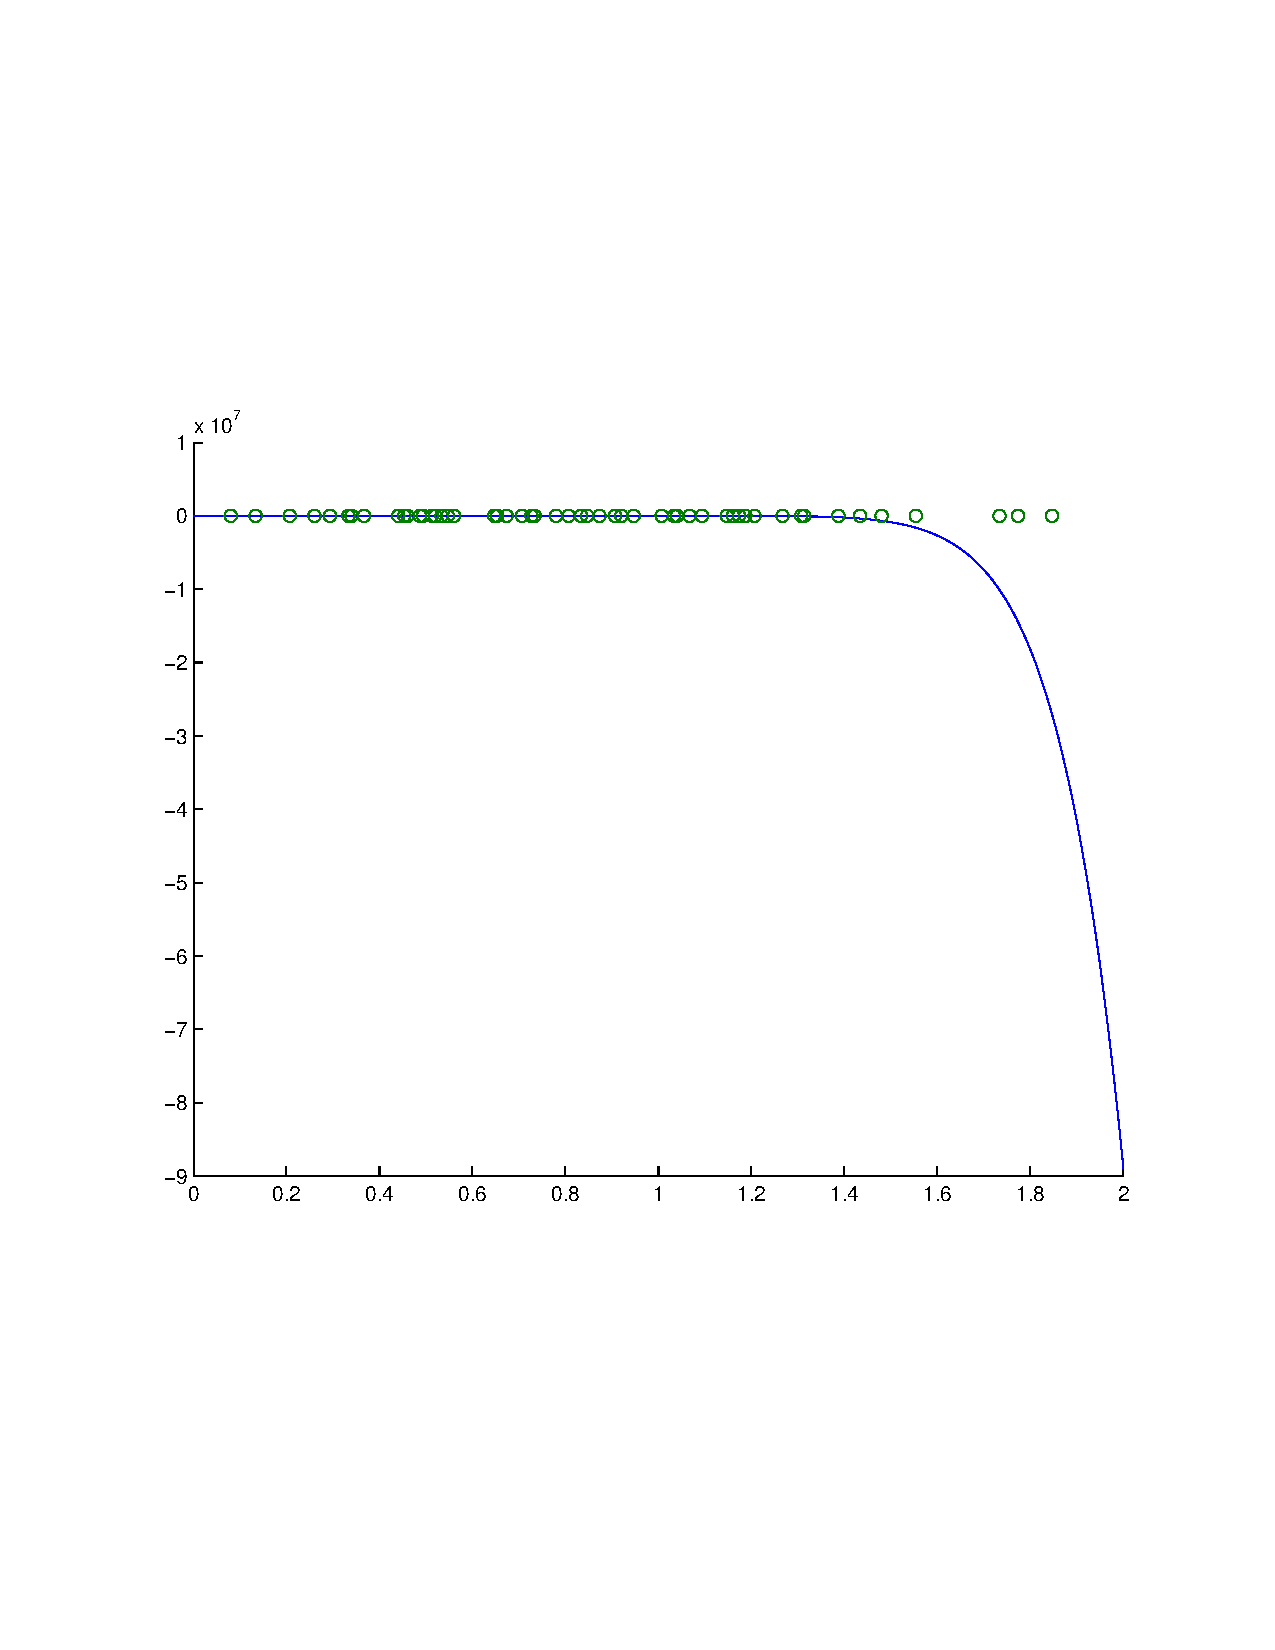
\includegraphics[width=.22\textwidth]{\figdir/prob1c_deg10} &
%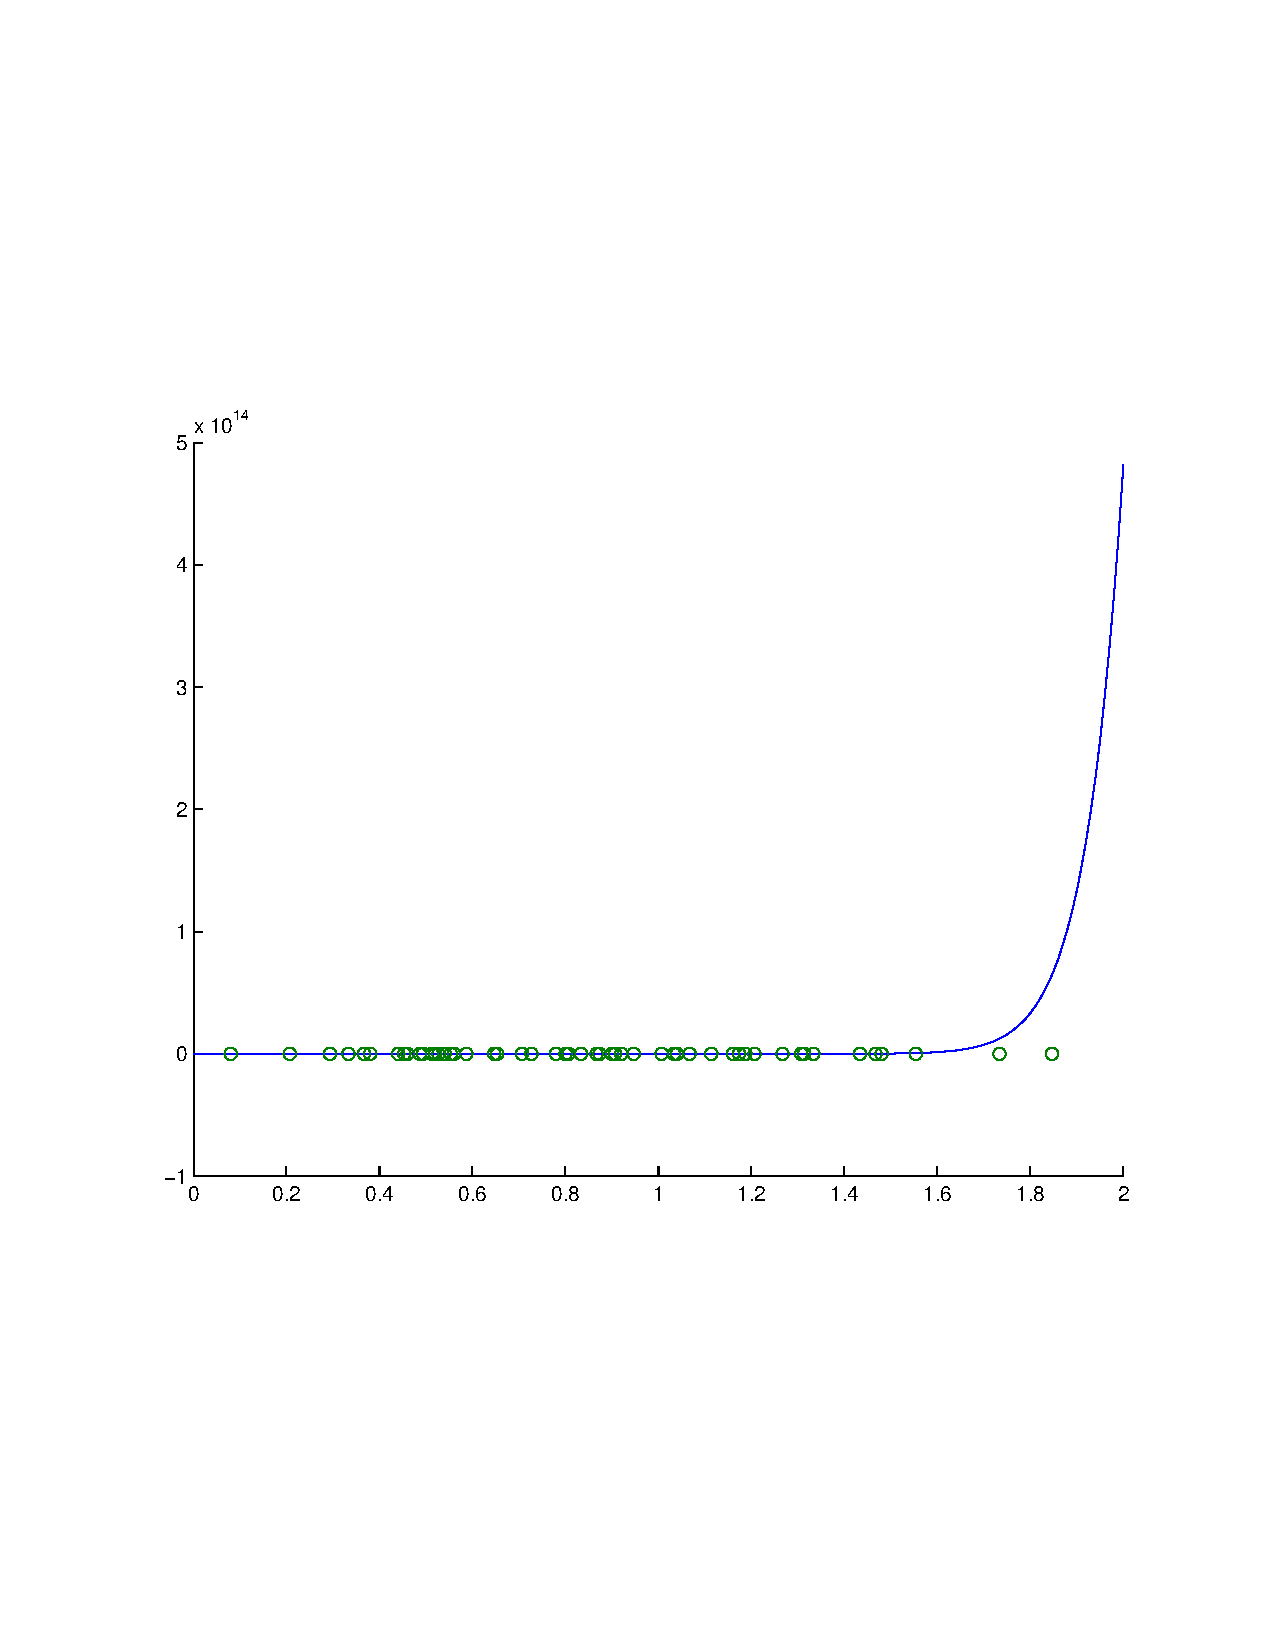
\includegraphics[width=.22\textwidth]{\figdir/prob1c_deg18} &
%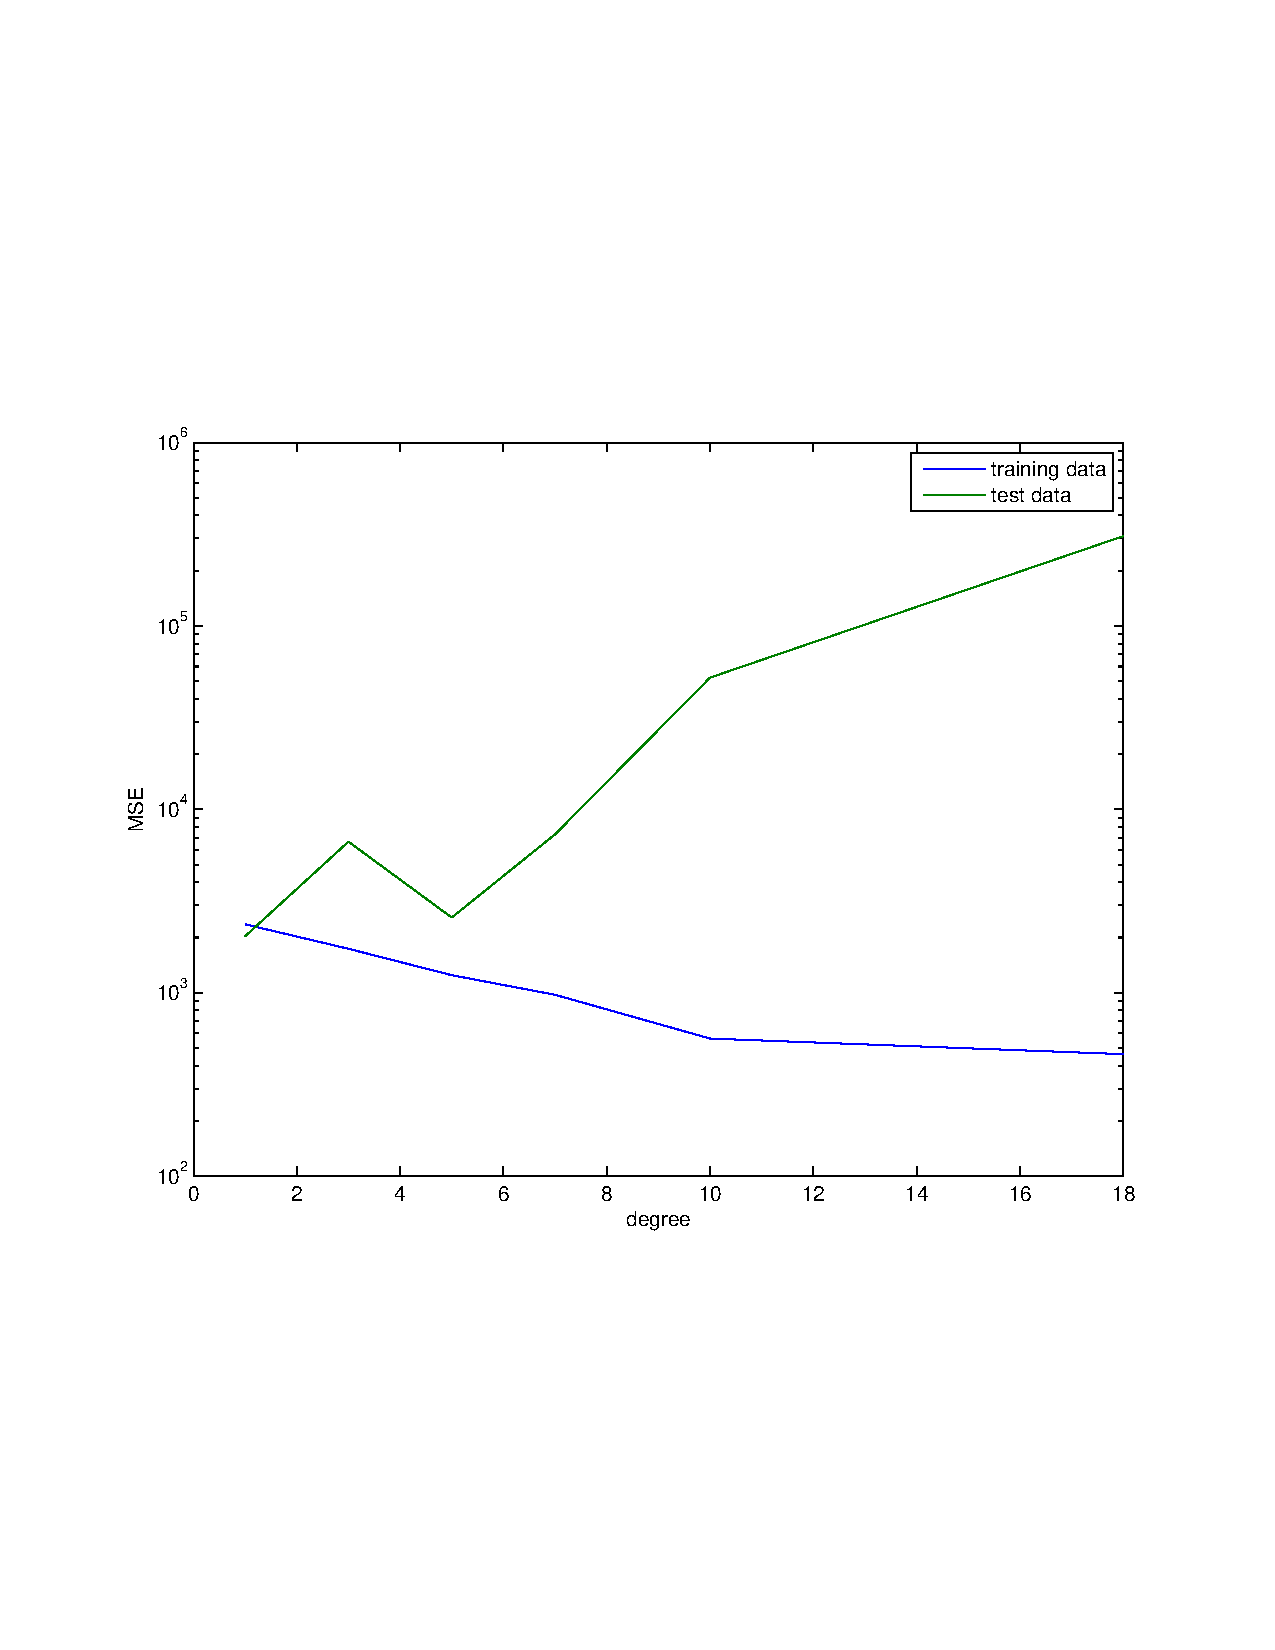
\includegraphics[width=.22\textwidth]{\figdir/prob1c_mse} \\
%10 & 18 & MSE
%\end{tabular}
%\end{figure}

\end{enumerate}

% % % % % % % % % % % % % % % % % % % % % % % % % % % % % % % % % % % % % % % % % % % % % % % % % % % % % % % % % % % % % % % %

\subsection*{Problem 2: k-means Clustering on Text}

\begin{enumerate}[(a)]
\item Done
\item Cost function results: 2.2505, 2.2706, 2.1498, 2.1769, 2.6815 \\
Cluster 1 has 22 articles \\
Most common words: y2k, 2000, system, computer, saturday, problem, problems, government, news, city, \\
Cluster 2 has 3 articles \\
Most common words: games, million, olympic, trump, city, griffey, donald, federal, age, stadium, \\
Cluster 3 has 1 articles \\
Most common words: air, airlines, friday, traffic, aviation, commercial, midnight, 2000, canceled, control, \\
Cluster 4 has 2 articles \\
Most common words: party, candidate, clinton, early, national, primary, republican, system, bad, bond, \\
Cluster 5 has 4 articles \\
Most common words: algeria, islamic, war, americans, country, army, europe, front, independence, called, \\
Cluster 6 has 3 articles \\
Most common words: white, mall, president, guests, house, clinton, dinner, crowd, millennium, room, \\
Cluster 7 has 5 articles \\
Most common words: greene, buildings, architecture, city, architects, hobson, maurice, kansas, landmark, company, \\
Cluster 8 has 1 articles \\
Most common words: sun, celebration, morning, saturday, town, american, hall, light, line, maine, \\
Cluster 9 has 3 articles \\
Most common words: y2k, saturday, problems, 2000, koskinen, computers, country, horn, operations, reported, \\
Cluster 10 has 1 articles \\
Most common words: patriots, deal, free, million, coaches, game, season, carroll, cap, coach, \\
Cluster 11 has 1 articles \\
Most common words: beamon, mother, book, jump, school, black, bob, died, family, sports, \\
Cluster 12 has 1 articles \\
Most common words: central, clouds, snow, states, valley, weather, week, air, band, century, \\
Cluster 13 has 1 articles \\
Most common words: look, mrs, feel, head, president, believe, story, women, clinton, considered, \\
Cluster 14 has 1 articles \\
Most common words: market, percent, growth, stocks, analysts, 2000, inflation, stock, 1999, economic, \\
Cluster 15 has 21 articles \\
Most common words: test, square, times, end, millennium, houston, fireworks, city, midnight, 2000, \\
Cluster 16 has 148 articles \\
Most common words: team, game, season, york, players, century, american, political, yeltsin, games, \\
Cluster 17 has 5 articles \\
Most common words: yards, game, bowl, texas, arkansas, season, yard, offensive, line, touchdown, \\
Cluster 18 has 2 articles \\
Most common words: susan, y2k, smiths, farm, call, food, going, jim, real, thing, \\
Cluster 19 has 2 articles \\
Most common words: bowden, coach, football, florida, field, players, head, assistant, practice, ann, \\
Cluster 20 has 1 articles \\
Most common words: hong, kong, 000, evening, horse, millennium, chinese, eve, midnight, party, \\

We can see that most of the clusters seem to have some sort of common theme between the words, though in some cases we may need to look at more words to discern what that is.
Interestingly, we see that some clusters should obviously be split again as they seem to have more than one theme, such as cluster 16 that seems to have documents about both sports as well as Russian politicians.

\item The documents seem to form somewhat coherent groups, though in some cases they seem to be members of clusters shared with other coherent groups.  
These do seem to be the best clusters for the documents given the spread of common words, though as previously mentioned the clusters could be rearranged to improve this match.

\item The sum of squared distances is \textbf{1.7278}, which is significantly lower than the previous clustering.
Now, the clusters seem to better match the documents contained within as the cluster containing documents about Russia seems to contain \emph{only} documents about Russia.
However, there certainly exists a problem with too many clusters as many clusters contain only 1 or a few articles, such as the sports article about Cal State Northridge.

%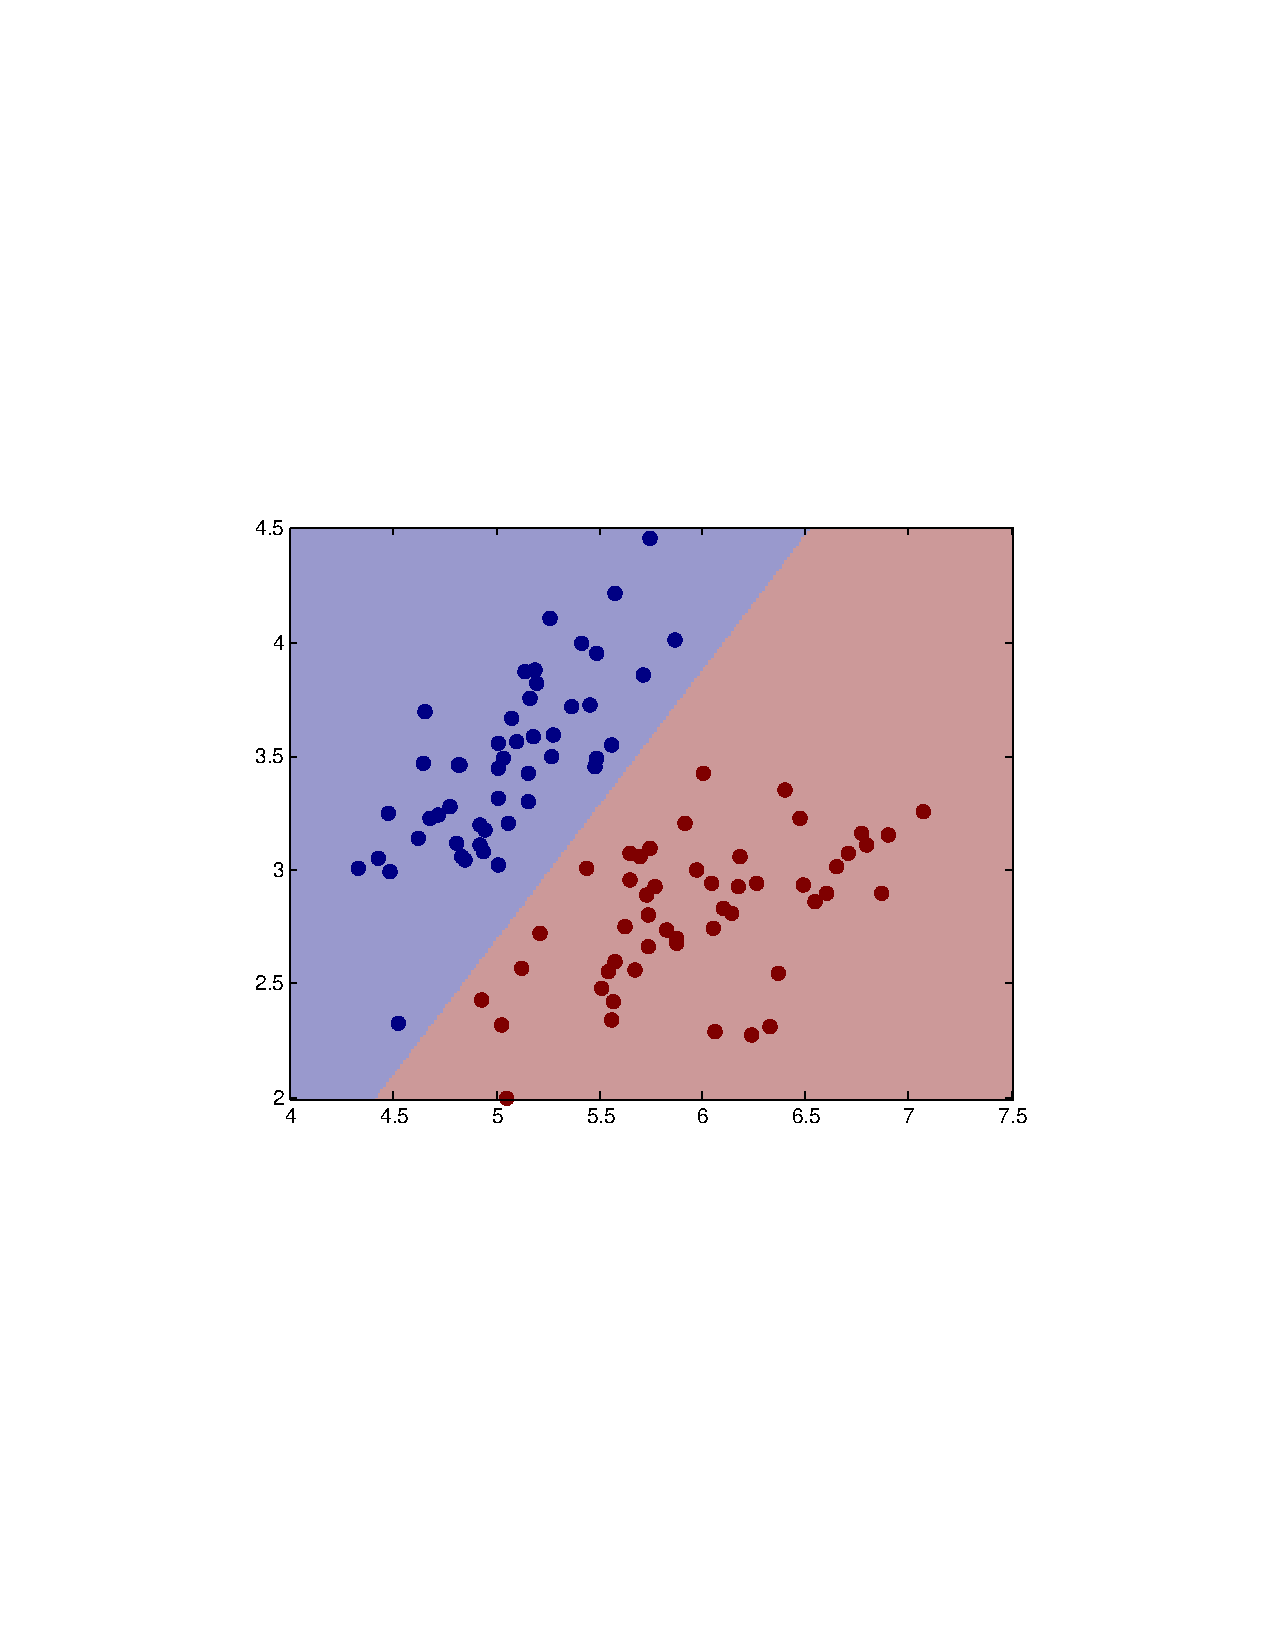
\includegraphics[width=.45\textwidth]{\figdir/prob2a}
\end{enumerate}

% % % % % % % % % % % % % % % % % % % % % % % % % % % % % % % % % % % % % % % % % % % % % % % % % % % % % % % % % % % % % % % %

\subsection*{Problem 3: EigenFaces}

\begin{enumerate}[(a)]
\item TODO
\end{enumerate}

% % % % % % % % % % % % % % % % % % % % % % % % % % % % % % % % % % % % % % % % % % % % % % % % % % % % % % % % % % % % % % % %

\subsection*{Problem 4: Project}

Yessir!

\end{document}
